\chapter{Projeto de implementação}
\label{cap:projetoimplementacao}

Neste capítulo serão apresentados os serviços considerados mais críticos para a empresa. Posteriormente, será proposta uma solução de implementação 
de alta disponibilidade para estes. Essa solução será detalhada na Seção \ref{section:propostasolucao}, e será baseada na utilização de 
virtualização e de \textit{softwares} de código aberto. 

\section{Levantamento dos serviços críticos}
\label{section:servcrit}

No capítulo anterior foram detalhados todos os serviços que estão disponíveis na empresa. Nesta seção será feito uma análise desses
serviços, destacando os serviços considerados mais críticos para a empresa. Para a seleção dos serviços críticos foram adotados os seguintes
critérios:
\begin{itemize}
 \item A quantidade de clientes ou funcionários que utilizam o serviço: esse é o item mais relevante, pois impacta diretamente no faturamento
 da empresa. De fato, se um cliente ficar sem acesso à Internet, o cliente terá um desconto proporcional ao tempo que ficou sem 
 acesso; 
 \item O número de requisições: esse número é importante, uma vez que, indicam a quantidade de usuários que dependem do serviço e a frequência
 de utilização do serviço. Esse critério engloba, por exemplo, o número de conexões \ac{TCP} \cite{tanenbaum2011} de um serviço, o número de 
 requisições \ac{UDP} \cite{tanenbaum2011}, a quantidade de acessos em um servidor de hospedagens de sites e a quantidade de requisições \ac{DNS} 
 em um servidor recursivo;
 \item O volume de elementos do serviço: essa medida demonstra a abrangência do serviço, ou seja, quantos clientes são dependentes deste. 
 Como exemplo de elementos pode-se citar a quantidade de contas ativas de \textit{e-mail} em um servidor de \textit{e-mail} ou a quantidade de 
 equipamentos monitorados por um servidor de monitoramento;
 %Esse critério é importante pois com ele pode-se comparar diferentes serviços possibilitando perceber o grau de relevância que cada um possui;
 %Esse critério, como o anterior, também permite comparar diferentes serviços para ter a possibilidade de ordená-los de acordo com sua relevância, por isso o torna importante para esta análise.
\end{itemize}

Nas próximas seções serão descritos os serviços críticos, com base nos critérios adotados.

\subsection{DNS recursivo primário}
\label{section:dnsrecprim}

Esse serviço foi classificado como o serviço mais importante pois possui um impacto direto nos clientes do provedor. Além disso, esse é o único 
serviço que todos os clientes e funcionários utilizam, totalizando aproximadamente 9000 pessoas. O objetivo de um provedor é fornecer uma navegação 
de qualidade aos seus clientes, sendo assim, o \ac{DNS} é fundamental para essa navegação, uma vez que é usado por todos os clientes. Outro 
importante critério que pode ser aplicado ao \ac{DNS} recursivo é o número de requisições por segundo. Como pode ser observado na Figura 
\ref{fig:dns_udp} (a) esse serviço possui picos de aproximadamente 1150 requisições por segundo. De acordo com a Figura \ref{fig:dns_udp} (b) 
pode-se observar que o servidor \textit{Passata} é o servidor que possui um maior número de requisições \ac{UDP}\footnote[1]{Esse número de 
requisições \ac{UDP} é elevado devido ao fato do serviço \ac{DNS} utilizar esse protocolo de transporte.}. Essa figura compara os principais 
servidores da empresa através de requisições \ac{UDP}, sendo que esse número de requisições indica a quantidade de clientes que utilizam os 
serviços.

\begin{figure}[h!]
 \centering
 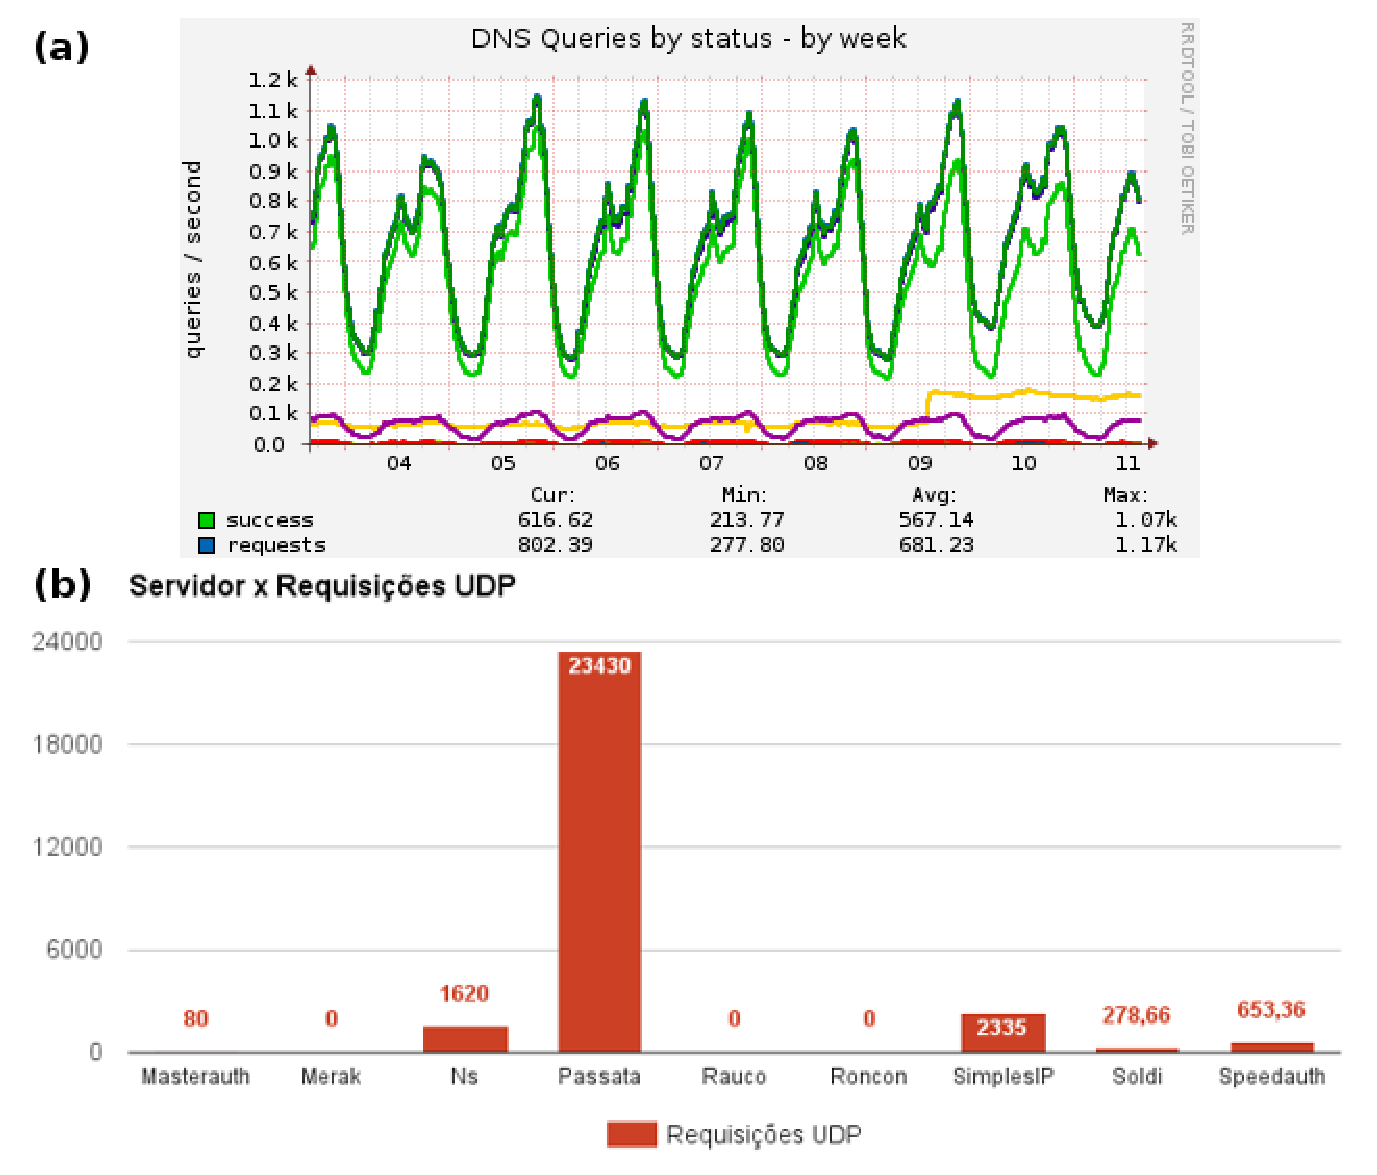
\includegraphics[width=400px]{img/dns_udp.eps}
 \caption{Gráfico de requisições DNS (a) e comparação de requisições UDP entre os principais servidores (b).}
 \label{fig:dns_udp}
\end{figure}

\subsection{Autenticação Radius}
\label{section:radius}

Esse serviço é importante pois é o responsável pela autenticação de todos os clientes do provedor. Caso esse serviço fique indisponível, 
os clientes não conseguirão estabelecer conexão e, consequentemente, não conseguirão utilizar o serviço de Internet. Os servidores 
\textit{Masterauth} e \textit{Speedauth} fornecem o serviço de \textit{Radius}, sendo que recebem, em média, 1,6 requisições de autenticação 
por segundo, como pode ser observado na Figura \ref{fig:freeradius_auth} (a) e na \ref{fig:freeradius_auth} (b). Caso esses servidores fiquem 
indisponíveis aproximadamente 2 clientes não conseguirão realizar a autenticação. Além disso, esses servidores armazenam dados relacionados à 
conexão dos clientes, como por exemplo, o endereço de \ac{IP} que é utilizado por um cliente em um determinado período de tempo, o tráfego de 
dados da conexão, o tempo da conexão de cada cliente, o endereço \ac{MAC} dos equipamentos dos clientes, entre outros. Essas operações resultam 
em média 23 requisições por segundo. %, como pode ser observado na Figura \ref{fig:speedauth_acct_week} e \ref{fig:masterauth_acct_week};
Outro critério que é relevante para esses servidores é o volume de elementos do serviço, que neste caso, representa a quantidade de clientes de
acesso à Internet. Como pode ser observado na Figura \ref{fig:elementos_tcp} (a), os servidores \textit{Masterauth} e \textit{Speedauth}
estão entre os que apresentam o maior número de elementos. Além disso, existem um grande número de conexões \ac{TCP} nesses servidores, como 
pode ser observado na Figura \ref{fig:elementos_tcp} (b).

\begin{figure}[h!]
 \centering
 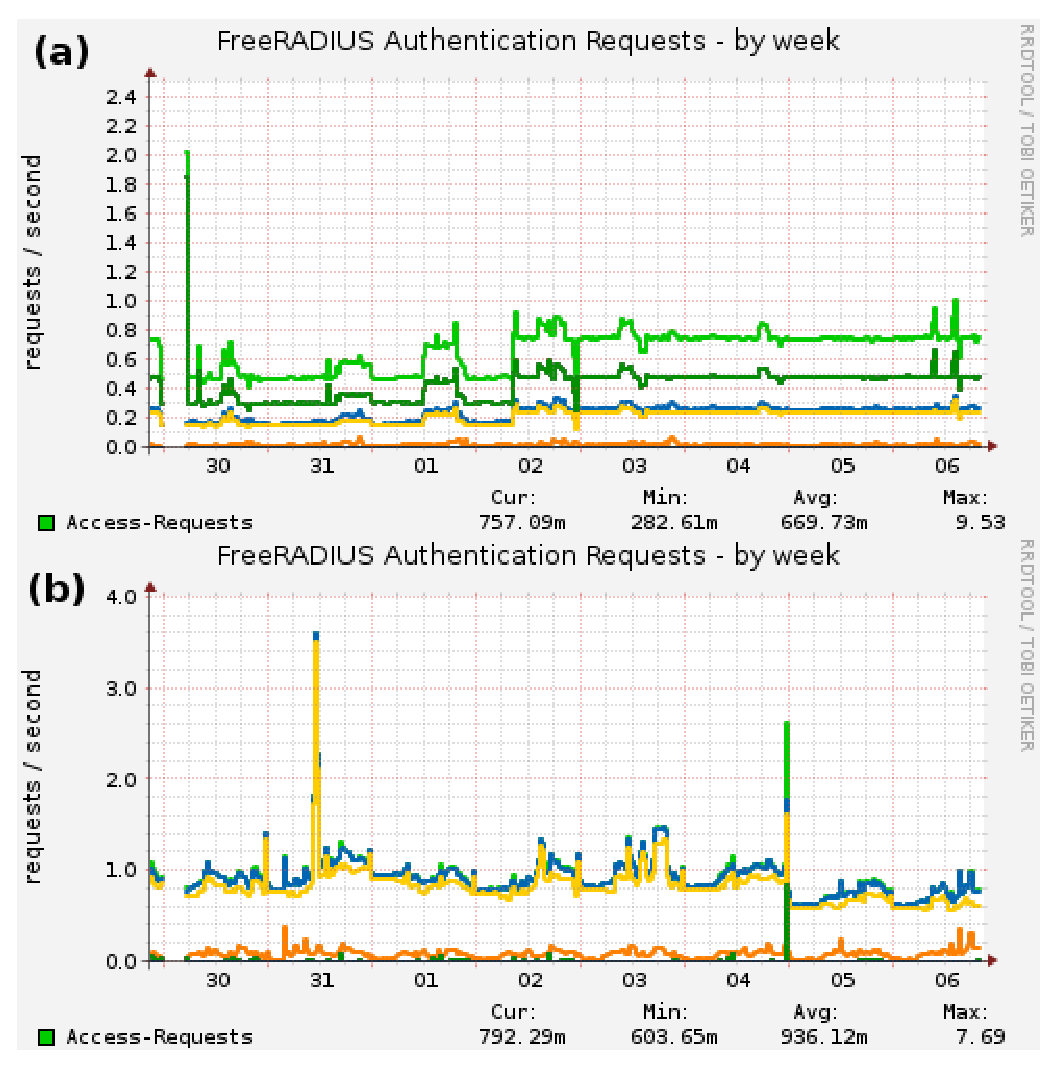
\includegraphics[width=300px]{img/freeradius_auth.eps}
 \caption{Gráfico de requisições de autenticação do servidor \textit{Masterauth} (a) e \textit{Speedauth} (b).}
 \label{fig:freeradius_auth}
\end{figure}

\begin{figure}[h!]
 \centering
 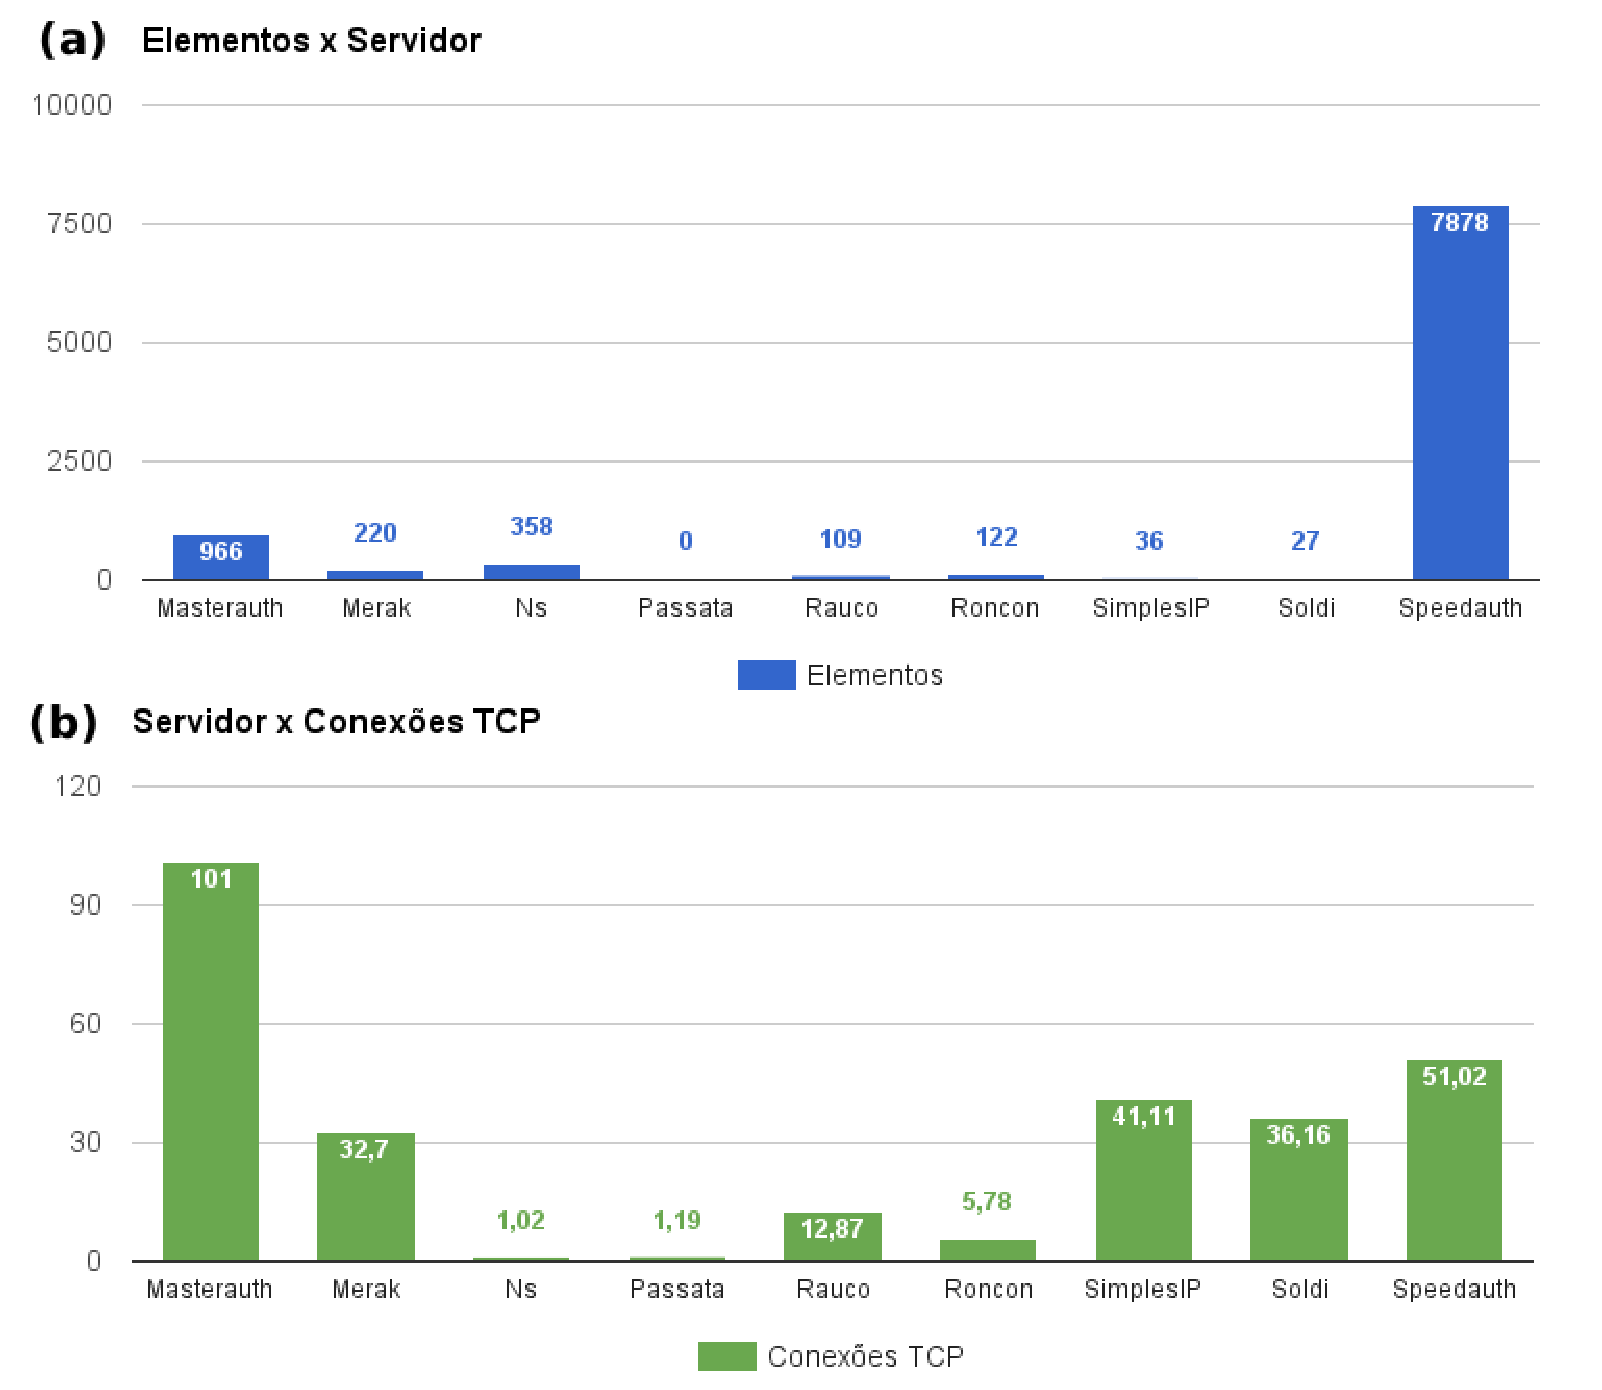
\includegraphics[width=380px]{img/elementos_tcp.eps}
 \caption{Gráfico de comparação de elementos (a) e de conexões TCP (b) entre os principais servidores.}
 \label{fig:elementos_tcp}
\end{figure}

\subsection{Sistemas da empresa e do provedor}
\label{section:sistemas}

O sistema do provedor é responsável pela maior parte das operações gerenciais do provedor. De fato, este sistema é responsável pela emissão de 
boletos, atendimento de clientes, comunicação interna da empresa, vendas, ativações de novos clientes, entre outros. Esse sistema não tem um 
impacto direto para os clientes, porém é fundamental para o funcionamento da empresa e do provedor. Caso haja uma indisponibilidade desses sistemas 
a maior parte dos funcionários ficarão impossibilitados de trabalhar, sendo que a empresa possui no total 65 funcionários.
%, sendo que são aproximadamente 35 funcionários simultâneos (de acordo com a Figura \ref{fig:ejabberd_week}), isso poderia gerar um prejuízo elevado para a empresa e o provedor. 
Esse sistema é executado no servidor \textit{Soldi} que recebe aproximadamente 3 requisições \textit{HTTP} \cite{tanenbaum2011} por segundo, como 
pode ser observado na Figura \ref{fig:soldi_week}. Além disso, a empresa mantém 28 sistemas de outros clientes nesse servidor. 
Também é importante destacar que esse serviço possui um número considerável de conexões \ac{TCP}, como pode ser observado na Figura 
\ref{fig:elementos_tcp} (b).

%\begin{figure}[h!]
% \centering
% 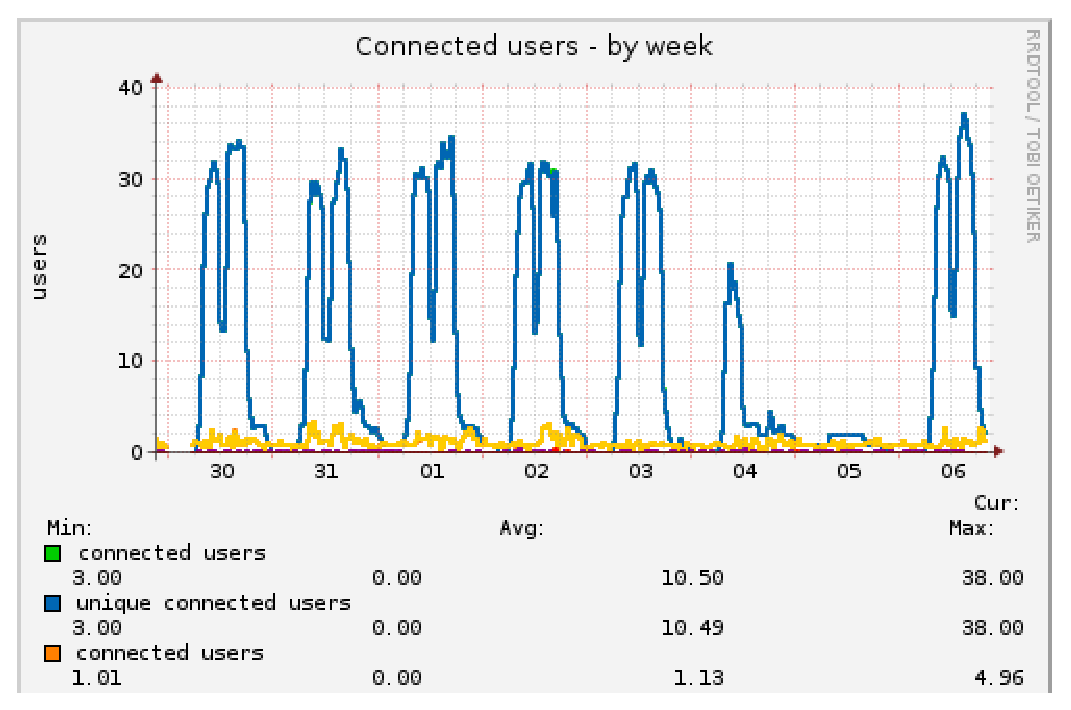
\includegraphics[width=310px]{img/ejabberd_week.eps}
% \caption{Gráfico usuários simultâneos de sistema.}
% \label{fig:ejabberd_week}
%\end{figure}

\begin{figure}[h!]
 \centering
 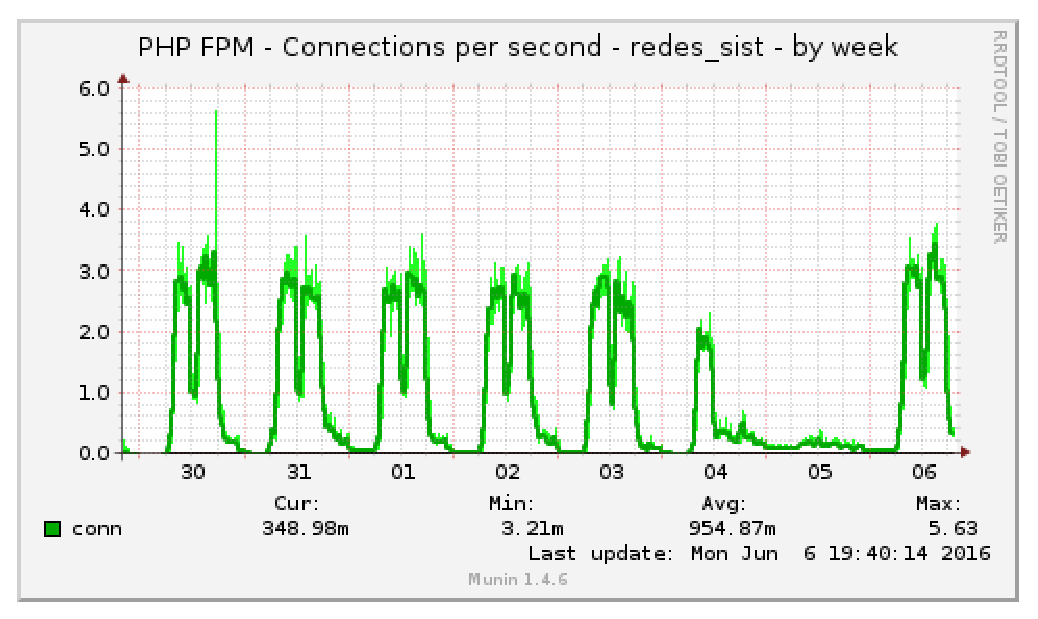
\includegraphics[width=300px]{img/soldi_week.eps}
 \caption{Gráfico de requisições por segundo do maior sistema.}
 \label{fig:soldi_week}
\end{figure}

\newpage
\subsection{Telefonia interna sobre IP}
\label{section:telefonia}

Esse serviço tem relevância para a empresa e para o provedor, pois permite a comunicação entre os clientes e os funcionários, ou seja, o 
servidor \textit{SimplesIP} é responsável por garantir o atendimento dos clientes para fins de suporte técnico, comunicação interna entre 
funcionários, comunicação com técnicos externos, vendas, cobranças a clientes, entre outros. Para quantificar, no mês de maio de 2016 a empresa 
recebeu 15922 ligações, com duração total de 67 horas e 40 minutos. Além disso, no mesmo mês foram efetuadas 674 ligações entre funcionários. 
O gráfico da Figura \ref{fig:simplesip_week} mostra a quantidade de canais ativos no servidor de telefonia. Observa-se nesta figura que ocorre 
de 20 a 30 ligações simultâneas durante o horário comercial, que é das 08:00 às 12:00 e das 13:00 às 18:00. Também pode-se observar, na Figura 
\ref{fig:dns_udp} (b), que esse serviço possui um elevado número de requisições \ac{UDP}\footnote[1]{Esse número de requisições \ac{UDP} 
deve-se ao fato da telefonia utilizar o protocolo \ac{UDP} para transmissão de voz.} comparado aos demais servidores.

\begin{figure}[h!]
 \centering
 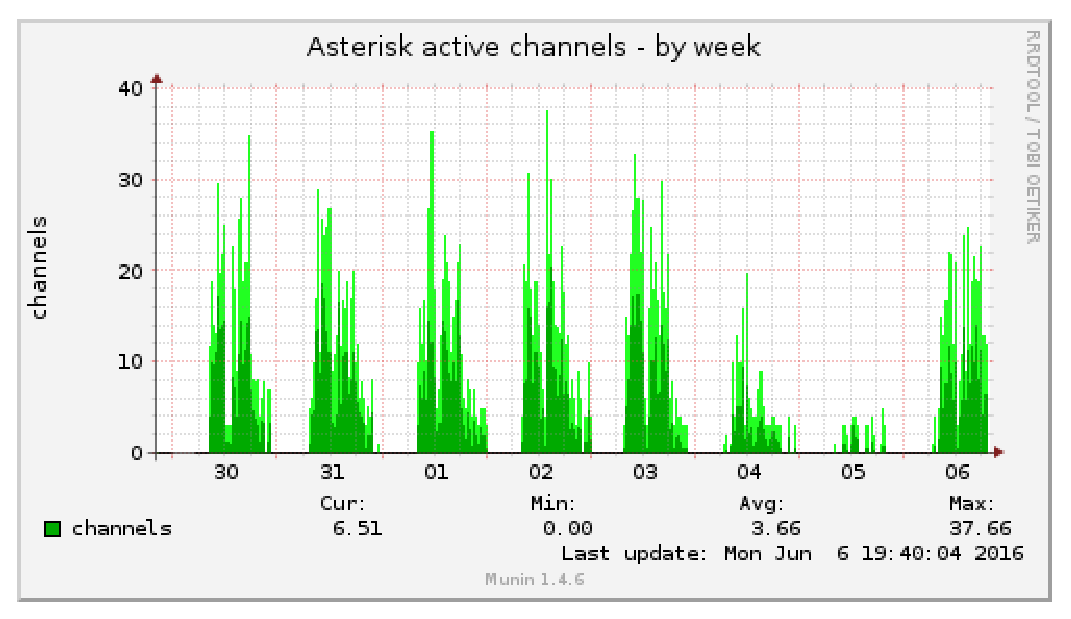
\includegraphics[width=300px]{img/simplesip_week.eps}
 \caption{Gráfico da quantidade de canais ativos no servidor de telefonia.}
 \label{fig:simplesip_week}
\end{figure}

\subsection{Situação atual}
\label{section:maqservcrit}

A partir da análise inicial, verificou-se que os servidores a serem incluídos no ambiente de alta disponibilidade são:
\begin{itemize}
 \item \textit{Passata}: servidor de \ac{DNS} recursivo utilizado tanto pelo provedor quanto pela empresa;
 \item \textit{Speedauth}: principal servidor \textit{Radius} para autenticação dos clientes do provedor;
 \item \textit{Masterauth}: segundo servidor \textit{Radius} para autenticação dos clientes do provedor;
 \item \textit{Soldi}: servidor de sistemas da empresa e do provedor;
 \item \textit{SimplesIP}: servidor de telefonia interna sobre \ac{IP} para atendimento aos clientes e comunicação interna do provedor e da empresa;
\end{itemize}

Na Tabela \ref{tab:dispservcrit}, tem-se esses servidores, seus respectivos serviços, o percentual de \textit{Uptime}\footnote[1]{O serviço de 
telefonia do servidor SimplesIP foi implantado em 06/2015, sendo assim sua medição é dos últimos 6 meses de 2016, por isso possui um 
\textit{Uptime} elevado.} e o tempo de \textit{Downtime} 
por ano. 

% subir pagina da tabela ??
\begin{table}[h!]
\caption{Serviços críticos do ano de 2015.}
\label{tab:dispservcrit}
\begin{center}
\begin{tabular}{|l|l|l|l|}\hline
\textbf{Servidor} & \textbf{Serviço} & \textbf{Uptime} & \textbf{Downtime por ano} \\\hline
Passata & DNS recursivo & 99,913\% & 7 horas 37 minutos 30 segundos \\\hline
Speedauth & Radius & 99,755\% & 21 horas 25 minutos 50 segundos \\\hline
Masterauth & Radius & 99,475\% & 33 horas 47 minutos \\\hline
Soldi & Sistemas & 99,989\% & 59 minutos 30 segundos \\\hline
SimplesIP & Telefonia & 99,997\% & 15 minutos 10 segundos \\\hline %simplesip-ping pois asterisk nao esta correto
\end{tabular}
\end{center}
\end{table}

A partir da implementação da solução de alta disponibilidade deste trabalho pretende-se atingir um \textit{Uptime} de 99,99\%.

\section{Proposta de solução}
\label{section:propostasolucao}

Para implementar esta solução será necessário dois servidores físicos, sendo que a configuração de cada servidor deverá ser de 
%real = 11 \textit{cores} de processamento, 12 GB de memória \ac{RAM} e 156 GB de disco rígido
12 \textit{cores} de processamento, 14 GB de memória \ac{RAM} e 180 GB de disco rígido. Essa configuração foi calculada a partir da soma dos 
recursos atuais das máquinas virtuais que possuem os serviços críticos, que foram apresentadas na Seção \ref{section:servcrit}.
Com essa solução, caso ocorra alguma falha em um servidor, as máquinas virtuais serão transferidas para o outro servidor.
Destaca-se que tais recursos já encontram-se disponíveis bastando efetuar uma reorganização das máquinas virtuais.

Já os \textit{softwares} necessários para a implementação da alta disponibilidade podem ser divididas em dois grupos, \textit{softwares} de 
replicação de dados e \textit{softwares} para o monitoramento e a transferências das máquinas virtuais entre os servidores.

\subsection{Softwares para a replicação de dados}
\label{section:toolrepl}

A replicação de dados pode ser realizada de diferentes formas, que podem ser a nível de aplicação ou até mesmo a nível de \textit{hardware}.
Dependendo do objetivo e da aplicação pode-se usar como, por exemplo, a forma de replicação em \textit{hardware} que é utilizada em discos, o 
\ac{RAID} \cite{tanenbaum2009sistemas}. Essa solução é eficaz para garantir que o sistema não fique indisponível em caso de falha de 
discos\footnote[2]{Lembrando que essa solução é utilizada no ambiente atual para aumentar a disponibilidade dos servidores.}, porém não garante 
a disponibilidade quando um \textit{software} ou algum outro componente de \textit{hardware} falhar \cite{zaminhani2008}.

A solução de replicação a ser adotada consiste em um espelhamento de dados através da rede. Essa solução permite a cópia dos dados de um servidor
para um servidor remoto em tempo real. Normalmente essa solução é estruturada na forma de \textit{cluster}\footnote[3]{Pode-se definir 
\textit{cluster} como um grupo de computadores interligador por rede com o objetivo de aumentar o desempenho ou disponibilidade de um serviço 
\cite{freitas2005}}.
As próximas seções irão detalhar os \textit{softwares} de replicação de dados que foram encontrados e estudados.

\subsubsection{Ceph RBD}
\label{section:cephrbd}
O \textit{Ceph RBD} \cite{cephrbd} faz parte do projeto \textit{Ceph} \cite{ceph}. O \textit{Ceph RBD} é responsável por prover acesso dos 
dispositivos de bloco que estão distribuídos ou replicados em um \textit{cluster}. Sua arquitetura é composta por um nó administrador, onde será
centralizado a gerência do \textit{cluster}, e deve conter no mínimo dois nós para armazenamento (\textit{Ceph OSD}) e monitoramento 
(\textit{Ceph Monitor}).
\cite{ceph}.

\subsubsection{DRBD}
\label{section:drbd}
O \ac{DRBD} \cite{drbd} é uma solução de replicação de dispositivos de armazenamento, que permite uma replicação de um dispositivo de bloco local 
para uma máquina remoto, implementado através de um módulo do \textit{kernel} \textit{Linux}. É um projeto de código aberto, é faz a replicação a 
nível de bloco, o que garante o sincronismo seguro dos dados. 

Para ilustrar, na Figura \ref{fig:drbd_basic} tem-se dois servidores com seus respectivos discos rígidos, \textit{hda1} e \textit{hda3}, formando 
um \textit{cluster}, sendo que esses discos estão sincronizados através da rede. Com isso, todas as operações de escritas realizadas no nó primário 
serão replicadas para o disco do nó secundário \cite{zaminhani2008}.

\begin{figure}[h!]
 \centering
 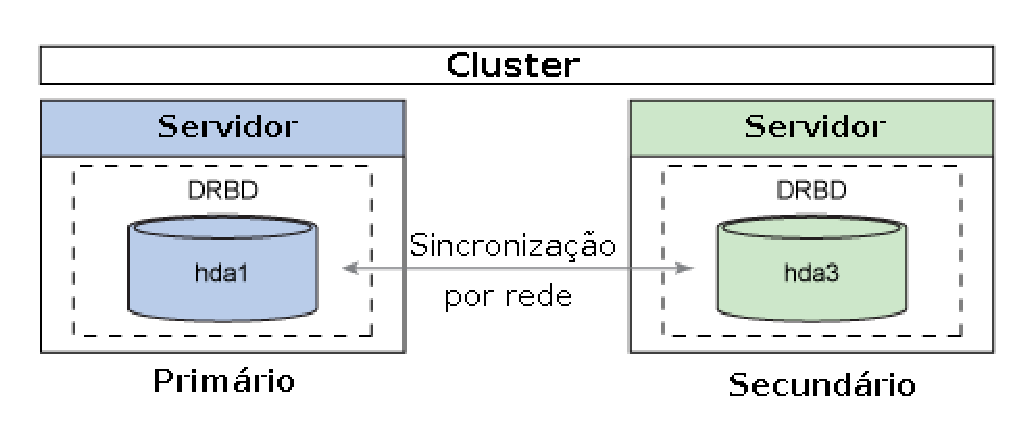
\includegraphics[width=300px]{img/drbd_basic.eps}
 \caption{Exemplo do modelo \textit{master-slave} do \ac{DRBD}.}
 Fonte: \citet{jones2010}
 \label{fig:drbd_basic}
\end{figure}

O \ac{DRBD} pode ser configurado dos seguintes modos \cite{drbd}:
\begin{itemize}
 \item \textit{Single-primary}: ou \textit{master-slave}, neste modo apenas um nó do \textit{cluster} pode ser o nó primário, sendo que esse nó 
 é o único que terá permissão para acessar o dispositivo, ou seja, somente ele poderá fazer operações de leitura e escrita. O nó 
 secundário apenas armazenará a réplica dos dados;
 \item \textit{Dual-primary}: ou \textit{dual-master}, neste modo existem dois nós primários, nos quais podem ser feitas operações de leitura e 
 escrita simultaneamente. Porém, este necessita de um sistema de arquivos compartilhados para fazer o gerenciamento das operações em arquivos, 
 pode-se citar o \ac{GFS} \cite{gfs} e o \ac{OCFS2} \cite{ocfs2} como exemplo desses sistemas de arquivos;
\end{itemize}

\subsubsection{GlusterFS}
\label{section:glusterfs}
O \textit{GlusterFS} \cite{glusterfs} é um sistema de arquivos distribuídos que utiliza a estrutura de \textit{cluster}. Sendo que, seu principal
objetivo é a escalabilidade, ou seja, existem uma facilidade para aumentar a capacidade do \textit{cluster}.
Ele também possui a opção de distribuição e replicação de dados, que caracteriza a alta disponibilidade \cite{glusterfs}.

\subsubsection{Rsync}
\label{section:rsync}
O \textit{Rsync} \cite{rsync} é um \textit{software} que sincroniza os servidores a partir de cópia dos dados de um servidor de origem 
para um de destino.

% Swift open stack
% https://wiki.freebsd.org/HAST

\subsubsection{Software de replicação escolhido}
\label{section:replicacaoescolhido}

A Tabela \ref{tab:replicacao} compara as ferramentas citadas anteriormente. Pode-se perceber que o \textit{Ceph RBD} não possui a opção de
\textit{master-slave}. Esse \textit{software} necessita de um \textit{hardware} adicional para sua administração, além de não ser uma escolha 
atrativa para um \textit{cluster} de pequeno porte devido a sua complexa configuração. 

Já o \textit{GlusterFS} poderia ser utilizado, porém ele faz a replicação a nível de arquivo, sendo assim, não é a ferramenta ideal para uma 
solução de alta disponibilidade utilizando virtualização. Além disso, sua principal característica, que é a escalabilidade\footnote[1]{A 
escalabilidade é a facilidade de aumentar a capacidade do \textit{cluster} a partir da inclusão de novos nós}, não será útil para esta 
implementação, pois esta implementado não requer um grande volume de dados.
E por fim, o \textit{Rsync} não pode ser utilizado pois não faz replicação em tempo real.

\begin{table}[h!]
\caption{Comparação ferramentas de replicação de dados.}
\label{tab:replicacao}
\begin{center}
\begin{tabular}{|l|p{2.7cm}|p{2.7cm}|p{2.7cm}|p{2cm}|}\hline
\textbf{Características} & \textbf{Ceph RBD} & \textbf{DRBD} & \textbf{GlusterFS} & \textbf{Rsync} \\\hline
Master-slave & Não & Sim & Sim & Não \\\hline
Replicação em tempo real & Sim & Sim & Sim & Não \\\hline
Nível de replicação & Bloco & Bloco & Arquivo & Arquivo \\\hline
Número máximo de nós & Ilimitado & 16 & 64 & Ilimitado \\\hline
Plataformas & CentOS, Red Hat, Debian, Fedora, Ubuntu & Suse, Debian, CentOS, Red Hat, Ubuntu & Debian, CentOS, Red Hat, Fedora, Ubuntu & Linux \\\hline
Integração com virtualização & Sim & Sim & Sim & Não \\\hline
\end{tabular}
\end{center}
\end{table}

Portanto, a ferramenta escolhida para replicação de dados na solução de alta disponibilidade desse trabalho foi o \ac{DRBD}, pois permite a 
configuração \textit{master-slave} ou \textit{dual-primary}, além de suportar a replicação de máquinas virtuais e fazer replicação a nível de 
bloco. Além disso, essa ferramenta possibilita fazer a resincronização dos dados automaticamente quando um nó retornar de uma falha 
ocorrida \cite{drbd}.

%https://www.reddit.com/r/linux/comments/1qwarp/drbd_vs_glusterfs/
% glusterfs mais escalavel, simples de administrar
% drbd melhor eficiencia(acredito) nivel de bloco, confiavel(10 anos develop)

% drbd: 2 nodes na versão 8 e 16 nodes por stacking / 16 nodes na versão 9

% drbd dispositivo primário e secundário zaminhani2008
% Segundo (ELLENBERG, 2007), a partir da versão 8 do DRBD é possível que,
%dependendo da aplicação, a execução ocorra em todos os nós do cluster
%simultaneamente (Ativo/Ativo). Para tornar isso possível é necessária a
%utilização de um sistema de arquivos exclusivo para cluster, como o OCFS2 6 e o
%GFS 7 por exemplo. Como a abordagem deste trabalho é cluster de alta
%disponibilidade, a utilização do DRBD no modo Ativo/Ativo não será discutida.

% glusterfs https://raobharata.wordpress.com/2012/10/29/qemu-glusterfs-native-integration/
% melhor performace com disco utilizando protocolo gluster file=gluster://path/to

% ceph http://docs.ceph.com/docs/master/start/intro/
% necessita minimo 3 monitores com osd, outra para administração
% precisa openstack + nova
% http://www.server-world.info/en/note?os=Ubuntu_14.04&p=ceph
% https://elkano.org/blog/live-migration-openstack-ubuntu-14-04/

\subsection{Softwares para o gerenciamento de cluster}
\label{section:toolcluster}

Para ser possível implementar uma solução de alta disponibilidade é necessário organizar os servidores em uma estrutura de \textit{cluster}.
Além disso, é necessário a utilização de \textit{softwares} que facilitam o gerenciamento desse \textit{cluster}. Esses \textit{softwares} 
permitem detectar falhas em um nó, ou seja, essas podem detectar falhas de \textit{hardware} e falhas de serviços. 
Essas ferramentas são conhecidas como \ac{CRM}. 

Após a detecção de uma falha, os \textit{softwares} de gerenciamento de \textit{cluster} executam algumas ações, entre elas estão o 
\textit{failover} e o \textit{failback}. O \textit{failover} é o processo no qual um servidor recebe os serviços que estavam executando em outro 
servidor que ficou indisponível. Esses \textit{softwares} executam também o processo de \textit{failback} que é o retorno dos serviços 
para o servidor de origem quando este ficar disponível. Esse ocorre após o \textit{failover} sendo que ele é opcional \cite{bassan2008}.

As próximas seções irão detalhar os \textit{softwares} de gerenciamento de \textit{cluster} que foram encontrados e estudados.

\subsubsection{Ceph}
\label{section:ceph}
O \textit{Ceph} \cite{ceph} é uma ferramenta para o armazenamento de dados distribuídos. Esta ferramenta tem foco em \textit{cluster} 
de armazenamento, sendo assim ela necessita de outra ferramenta para gerenciar as máquinas virtuais, como por exemplo \textit{OpenStack} 
\cite{openstack}. Sua arquitetura é composta por um nó administrador, onde será centralizado a gerência do \textit{cluster}, e no mínimo dois 
nós para fazer o armazenamento (\textit{Ceph OSD}), o monitoramento (\textit{Ceph Monitor}) e o processamento (\textit{Ceph MDS}) \cite{ceph}.

\subsubsection{Ganeti}
\label{section:ganeti}
O \textit{software} \textit{Ganeti} \cite{ganeti} é um gerenciador de \textit{cluster} de virtualização, sendo que foi desenvolvido 
especificamente para virtualização e suporta os hipervisores \ac{KVM} \cite{kvm} e \textit{Xen} \cite{xen}. Para sua implementação é necessário
um nó \textit{master}, para armazenar as configurações e gerenciar o \textit{cluster}, e um nó \textit{master candidate}, para o caso do 
nó \textit{master} falhar. Além disso, ele permite a criação de vários nós \textit{slaves}. As máquinas virtuais são chamadas de instâncias, 
sendo que em cada instâncias é configurado qual será o nó primário que essa executará e qual será o nó secundário dessa instância.

As principais funções desse \textit{software} são \cite{ganeti}:
\begin{itemize}
 \item Gerenciamento de armazenamento;
 \item Criação de instâncias, que são os sistemas operacionais convidados;
 \item Iniciar e finalizar máquinas virtuais, além de efetuar o \textit{failover} entre os servidores hospedeiros.
\end{itemize}

Na Figura \ref{fig:ganeti_arquitetura} tem-se a arquitetura deste \textit{software}. O \textit{cluster} é composto por nós, que por sua vez 
possuem instâncias (máquinas virtuais). As instâncias podem ser migradas manualmente de um nó para outro e também serão migradas no processo de
\textit{failover}. Caso o nó \textit{master} falhar, suas funções serão transferidas para o \textit{master failover} ou \textit{master candidate}.

\begin{figure}[h!]
 \centering
 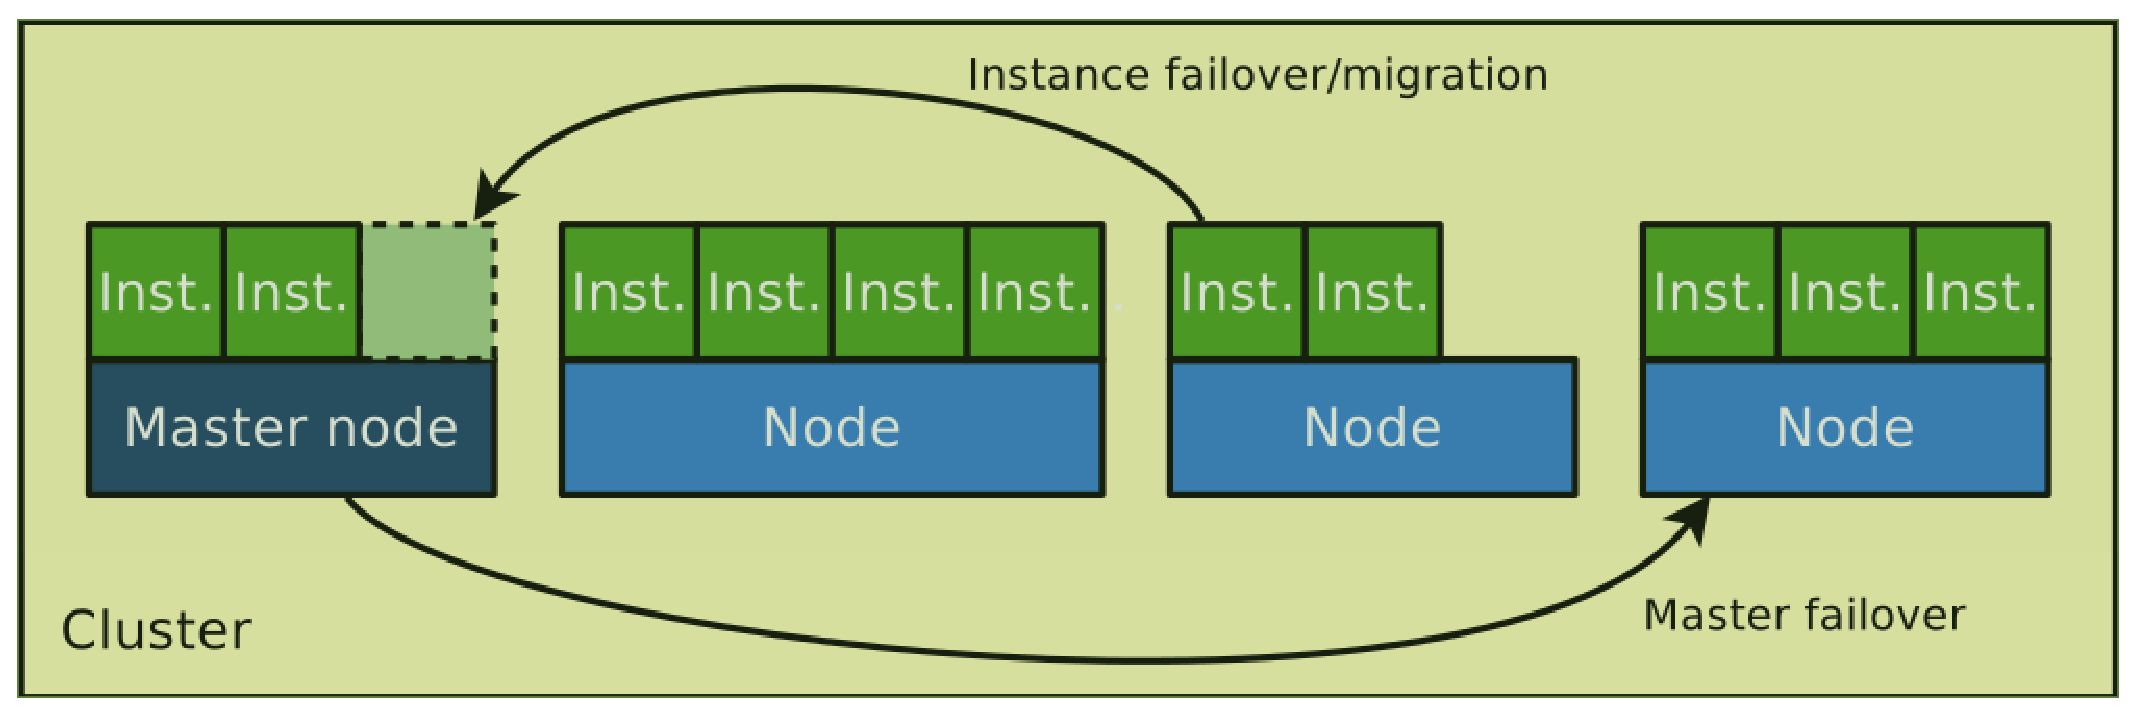
\includegraphics[width=340px]{img/ganeti_arquitetura.eps}
 \caption{Arquitetura do \textit{Ganeti}.}
 Fonte: \citet{carvalho2011}
 \label{fig:ganeti_arquitetura}
\end{figure}

% ganeti pode ser usado com ceph rdb (RADOS Cluster), ou drbd, ou gluster

\subsubsection{Heartbeat}
\label{section:heartbeat}
O \textit{Heartbeat} é um subprojeto do \textit{Linux-HA} \cite{linuxha}, que desenvolve aplicações para soluções de alta disponibilidade.
Esse subprojeto é uma aplicação que envia pacotes \textit{keepalive \ac{UDP}}, através da rede, para outras instâncias do \textit{Heartbeat}, 
com o objetivo de informar se ele está ativo \cite{reis2009}.

\subsubsection{Pacemaker}
\label{section:pacemaker}
O \textit{Pacemaker} \cite{pacemaker} pode ser definido como uma ferramenta de recuperação de falhas a nível de serviço \cite{perkov2011}. 
Esse \textit{software} é um projeto de código aberto mantido pela \cite{clusterlabs}, e teve origem com a necessidade de aperfeiçoar o gerenciador 
de recursos da ferramenta \textit{Heartbeat} \cite{heartbeat}, que possuía algumas limitações. 

Esse \textit{software} funciona juntamente com ferramentas que fazem troca de mensagens entre os nós do \textit{cluster} e ferramentas que 
fazem a afiliação, ou seja, fazem o processo de registro dos nós, de \textit{failover} e de bloqueios distribuídos, quando utilizado sistema 
de arquivos distribuídos. As ferramentas que podem ser integradas com o \textit{Pacemaker} são \cite{pacemaker}:
\begin{itemize}
 \item \textit{Corosync} \cite{corosync}: é responsável pelo processo de registro dos nós, de \textit{failover} e de bloqueios distribuídos 
 (utilizados para implementar \ac{LVM} \cite{lvm}, \ac{GFS}, e \ac{OCFS2}), entre outros. Essa ferramenta derivou do projeto \textit{OpenAIS};
 \item \textit{Heartbeat}: é um mecanismo que faz envio de mensagens entre os nós do \textit{cluster} com objetivo de notificar esse 
 \textit{cluster} quando houver alguma alteração de estado dos recursos ou dos nós, além de fazer o \textit{failover} \cite{clusterlabs}.
\end{itemize}
% outras ferramentas cMAN e Apache Qpid

%Modelos Active/Passive, N+1, N TO N, Split Site ??

Na Figura \ref{fig:pacemaker_tools} tem-se a arquitetura do \textit{Pacemaker}. Como pode ser observado na camada inferior tem-se os nós do 
\textit{cluster}. Acima as ferramentas de envio de mensagens, acima delas fica o \textit{Pacemaker}. Por fim, o \textit{DRBD}, o sistema de 
arquivos e os serviços do servidor.

\begin{figure}[h!]
 \centering
 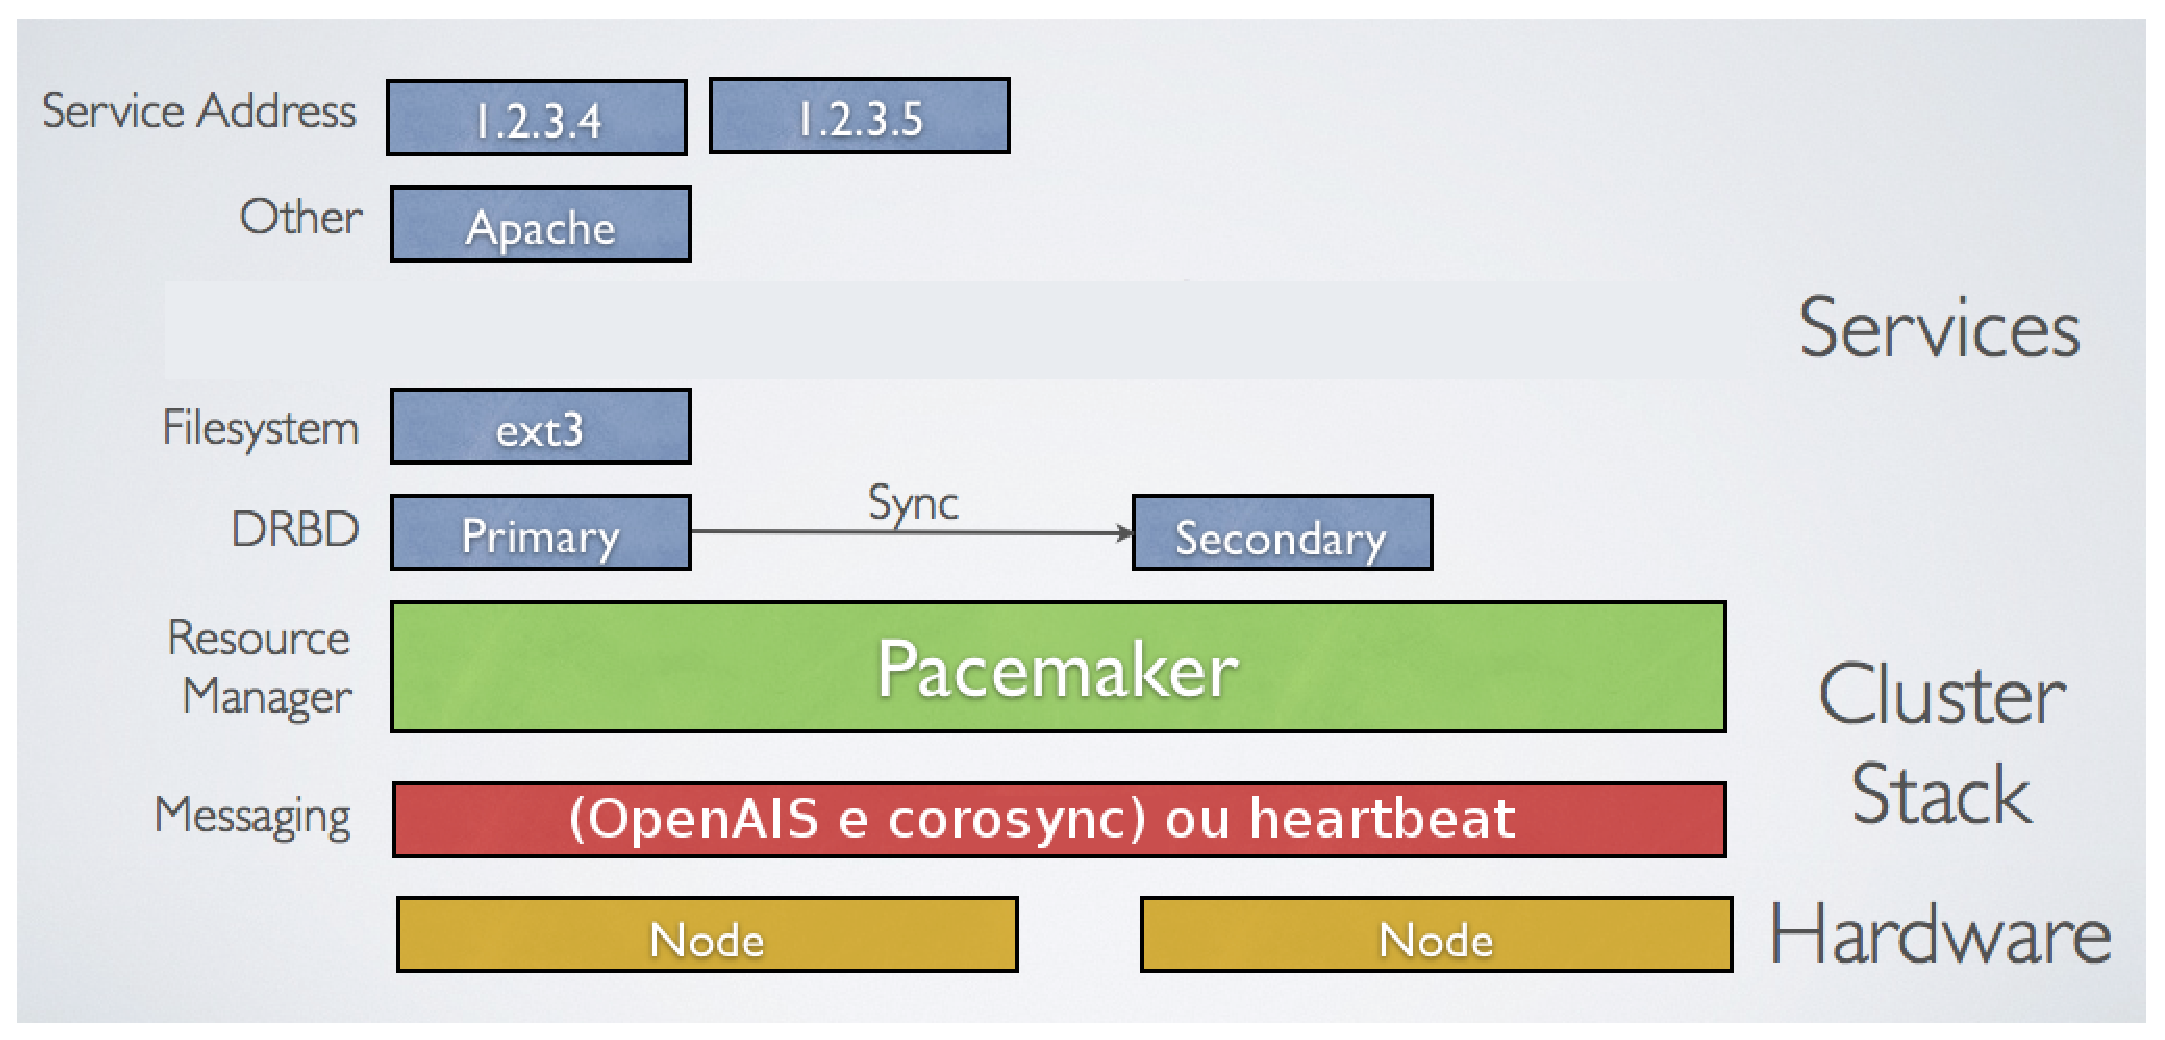
\includegraphics[width=300px]{img/pacemaker_tools.eps}
 \caption{Exemplo da arquitetura do \textit{Pacemaker}.}
 Fonte: \citet{pacemaker}
 \label{fig:pacemaker_tools}
\end{figure}

O \textit{Pacemaker} possui algumas funções principais que estão listadas abaixo:
\begin{itemize}
 \item Inicia e finaliza serviços dos nós do \textit{cluster}. Esses serviços podem ser desde um servidor \textit{web} até uma interface de 
 rede, por exemplo;
 \item Replica a configuração do \textit{cluster} para todos os nós de forma transparente, com isso a configuração de todo o \textit{cluster} 
 pode ser feita em qualquer nó;
 \item Elege um nó como primário para centralizar todas as decisões, sendo que, se esse nó falhar outro será eleito primário.
\end{itemize}

% Corosync provides pacemaker:
% a mechanism to reliably send messages between nodes,
% notifications when machines appear and disappear
% a list of machines that are up that is consistent throughout the cluster 
% Heartbeat provides:
% a mechanism to reliably send messages between nodes,
% notifications when machines appear and disappear
% a list of machines that are up that is consistent throughout the cluster 
% --
% http://serverfault.com/questions/269831/relation-between-heartbeat-openais-corosync
% well i reached answer on myself! clustering include two part:
% 1.cluster resource management
% 2.infrastructure with massaging layer
% legacy heartbeat is broken into heartbeat message layer and pacemaker so pacemaker is CRM.
% and we have two option on message layer:heartbeat,openais. openais/corosync is preferred as: http://comments.gmane.org/gmane.linux.highavailability.user/32355
% There are, however, features in Pacemaker that require OpenAIS which will work only with Corosync, not Heartbeat. Those features are concerned 
% with the distributed lock managers used by cLVM (but not regular LVM), GFS/GFS2, and OCFS2. If you need that functionality, you must select 
% OpenAIS/Corosync. If you do not, you're free to choose.
% as: http://www.clusterlabs.org/wiki/FAQ
% Originally Corosync and OpenAIS were the same thing. Then they split into two parts... the core messaging and membership capabilities are now 
% called Corosync, and OpenAIS retained the layer containing the implementation of the AIS standard.
% Pacemaker itself only needs the Corosync piece in order to function, however some of the applications it can manage (such as OCFS2 and GFS2) 
% require the OpenAIS layer as well.
% so i went to openais/corosync and integrate it with pacemaker.
% --
% There are, however, features in Pacemaker that require OpenAIS which
% will work only with Corosync, not Heartbeat. Those features are
% concerned with the distributed lock managers used by cLVM (but not
% regular LVM), GFS/GFS2, and OCFS2. If you need that functionality, you
% must select OpenAIS/Corosync.
% 
% Pacemaker itself only needs the Corosync piece in order to function, however some of the applications it can manage 
% (such as OCFS2 and GFS2) require the OpenAIS layer as well. 

\subsubsection{Software de gerenciamento escolhido}
\label{section:gerenciadorescolhido}

A Tabela \ref{tab:clusterger} compara alguns \textit{softwares} de gerenciamento de \textit{cluster} de acordo com algumas características. 
Pode-se observar que o \textit{software} \textit{Ceph} possui apenas detecção e recuperação a nível de nó. Esse \textit{software} tem foco 
em \textit{cluster} de armazenamento, desta forma ele necessita de outra ferramenta para gerenciar as máquinas virtuais, tornando assim sua 
configuração mais complexa. Além disso, essa ferramenta necessita de um \textit{hardware} especifico para administração do \textit{cluster}.

É possível também implementar uma solução de alta disponibilidade com a ferramenta \textit{Heartbeat}. Porém, desta forma seria necessário criar 
um conjunto de \textit{scripts} para fazer a migração das máquinas virtuais, o que dificultaria a implementação.

Já o \textit{Pacemaker} é o único que possui a característica de sincronismo de configuração entre todos os nós, no entanto, isto não é um 
grande diferencial. Devido ao monitoramento a nível de recurso, a ferramenta torna-se flexível para execução com diversas aplicações em 
diferentes ambientes, porém, nos testes efetuados em um ambiente de virtualização obteve-se dificuldade para concluir a implementação, pois a 
configuração tornou-se complexa.
%Pode-se observar que o \textit{Ganeti} não faz sincronismo das configurações, assim essas configurações devem ser feitas no nó \textit{master}.
%Porém, possui a vantagem de ser desenvolvido especificamente para virtualização. 

\begin{table}[h!]
\caption{Comparação ferramentas de gerenciamento de \textit{cluster}.}
\label{tab:clusterger}
\begin{center}
\begin{tabular}{|p{3.5cm}|p{2.7cm}|p{2cm}|p{2.7cm}|p{2.7cm}|}\hline
\textbf{Características} & \textbf{Ceph} & \textbf{Ganeti} & \textbf{Heartbeat} & \textbf{Pacemaker} \\\hline
Sincronismo de configuração entre os nós & Não & Não & Não & Sim \\\hline
Failover e failback & Não & Sim & Não & Sim \\\hline
Nível de detecção e recuperação & Nó & Nó e máquina virtual & Nó & Nó e recurso \\\hline
Plataformas & CentOS, Debian, Fedora, Red Hat, Ubuntu & Linux & Red Hat, CentOS, Fedora, Suse, Debian, Ubuntu & Red Hat, CentOS, Fedora, Suse, Debian, Ubuntu \\\hline
Integração com virtualização & Sim & Sim & Sim & Sim \\\hline
\end{tabular}
\end{center}
\end{table}

O \textit{software} escolhido para gerenciar o ambiente de alta disponibilidade, que será criado neste trabalho, foi a ferramenta de código aberto 
\textit{Ganeti}. Esse \textit{software} possui todos os requisitos para criar um \textit{cluster} de alta disponibilidade, além de possuir a 
vantagem de ser desenvolvido especificamente para virtualização, o que simplifica a sua configuração. O \textit{Ganeti} possui detecção de falhas 
tanto a nível de nó quanto a nível de máquina virtual. Nos testes realizados destaca-se a opção a migração em tempo real, pois obteve-se um bom 
resultado. Além disso, percebeu-se uma maior simplicidade na configuração do \textit{cluster}.
% O \textit{software} escolhido para gerenciar o ambiente que será criado neste trabalho foi a ferramenta de código aberto \textit{Pacemaker}. 
% Esse \textit{software} possui todos os requisitos para criar um \textit{cluster} de alta disponibilidade, sendo que, também pode ser configurada 
% para fazer monitoramento e recuperação tanto a nível de nó quanto a nível de recurso. Além disso, ela possui a característica de sincronismo de 
% configuração entre todos os nós que é exclusiva. Destaca-se que essa ferramenta é indicada no site do \ac{DRBD} para compor um \textit{cluster} 
% de alta disponibilidade \cite{drbd}.

\subsection{Projeto de implementação}
\label{section:projetoimpl}

Tendo todas as definições e ferramentas necessárias, pode-se criar o ambiente de alta disponibilidade, que é o objetivo deste trabalho.
Como mencionado anteriormente, esse ambiente será configurado na forma de um \textit{cluster} o qual será composto por no mínimo dois servidores, 
%real = 11 \textit{cores} de processamento, 12 GB de memória \ac{RAM} e 156 GB de disco rígido
com configuração de 12 \textit{cores} de processamento, 14 GB de memória \ac{RAM} e 180 GB de disco rígido. Essa configuração inclui
2 GB de memória \ac{RAM} e 24 GB de disco para cada sistema operacional dos servidores hóspedes. Além disso, será mantido o mesmo sistema 
operacional e o mesmo hipervisor utilizado no ambiente atual da empresa, o sistema \textit{Ubuntu 14.04 \ac{LTS}} e o \ac{KVM} \cite{kvm} 
respectivamente.

A nova estrutura desses servidores juntamente com suas máquinas virtuais e seus respectivos serviços estão contidos na Figura 
\ref{fig:projeto_estrutura}. Além disso será utilizado dois \textit{softwares}, o primeiro será o \ac{DRBD}, que fará a replicação dos dados 
das máquinas virtuais. Como pode ser observado na Figura \ref{fig:projeto_estrutura}, para cada \ac{VM} existe um disco \ac{DRBD} primário, 
sendo que este esta replicado em um disco secundário que está localizado no nó oposto do \textit{cluster}. O segundo \textit{software} será o 
\textit{Ganeti}, que fará o gerenciamento do \textit{cluster} e está localizado abaixo dos nós na Figura \ref{fig:projeto_estrutura}.

\begin{figure}[h!]
 \centering
 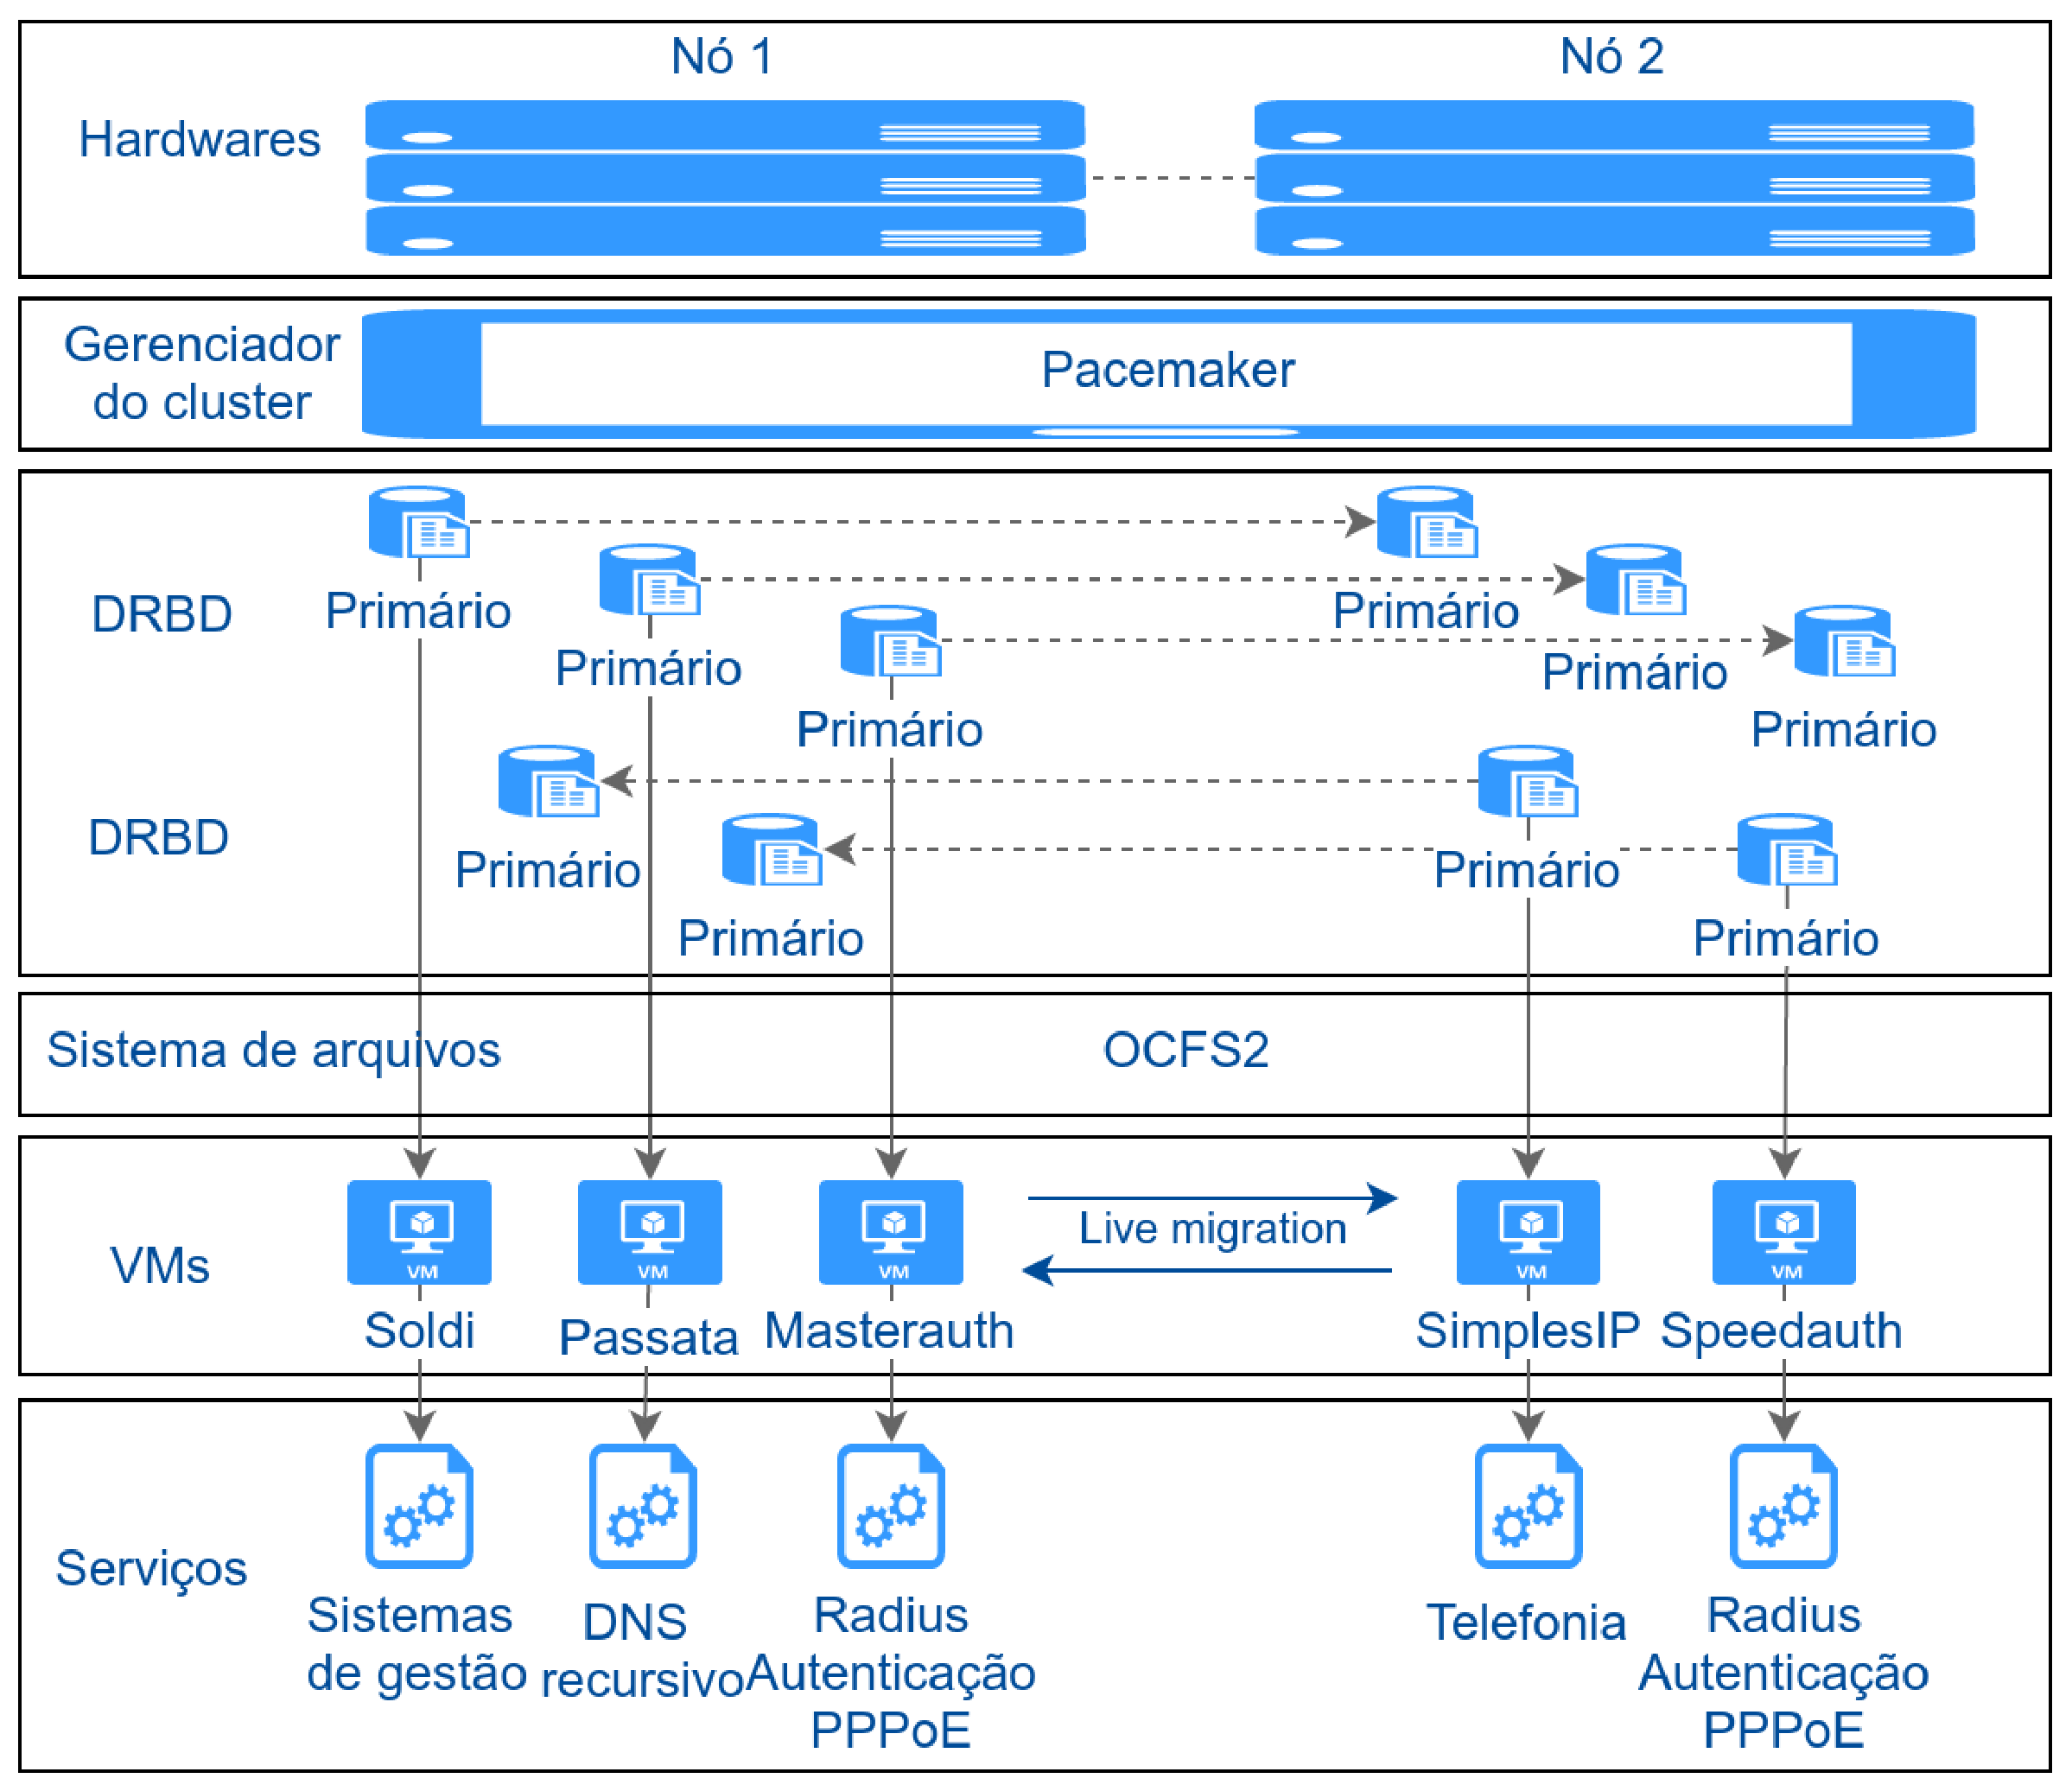
\includegraphics[width=380px]{img/projeto_estrutura.eps}
 \caption{Estrutura do \textit{cluster}.}
 \label{fig:projeto_estrutura}
\end{figure}

%drbd
O \ac{DRBD} será configurado no modo \textit{master-slave}, sendo que para cada disco das máquinas virtuais será criado um dispositivo de 
replicação \ac{DRBD}. E para utilizar esse dispositivo como disco de uma máquina virtual será criado um volume lógico 
\ac{LVM}\footnote{LVM é uma ferramenta de código aberto que possibilita a manipulação de discos rígidos, através da criação de grupos de volumes 
e volumes lógicos para \textit{Linux}.} \cite{lvm}. 

%ganeti
O \textit{software} \textit{Ganeti} será responsável pela gerência, monitoramento, \textit{failover}, migração das \ac{VM}s e criação das \ac{VM}s 
no \textit{cluster}. Para essas operações deve-se escolher um nó, que será o nó \textit{master}. Neste nó, primeiramente será feita inicialização 
do \textit{cluster}, ou seja, será feito a criação das configurações iniciais do nó \textit{master}. Essas configurações serão, por exemplo, 
a interface de rede, o \ac{IP}, o grupo de volumes do \ac{LVM} que o \textit{cluster} utilizará, entre outros. Após isso, será adicionado o outro 
nó para completar o \textit{cluster} e permitir a tolerância a falhas das máquinas virtuais. Por fim, será criado as instâncias, sendo que para 
cada instância será definido qual será o nó primário e o nó secundário. Essa instância criará um volume lógico \ac{LVM} nos dois nós, este será
o disco da máquina virtual. Desta forma, quando houver uma falha no nó primário a instância será migrada para o nó secundário, sem que a máquina 
virtual seja reiniciada.

Para essa migração, o \textit{Ganeti} utilizará a opção de migração em tempo real, mais conhecida como \textit{live migration}, que é fornecida 
pelo hipervisor \ac{KVM} \cite{kvm}. A Figura \ref{fig:vms_migration} demonstra dois servidores com um hipervisor e duas \ac{VM}s executando. 
Inicialmente estas estão executando sobre o primeiro servidor, então a \ac{VM} 1 é migrada para o segundo servidor \cite{livemigration}.

\begin{figure}[h!]
 \centering
 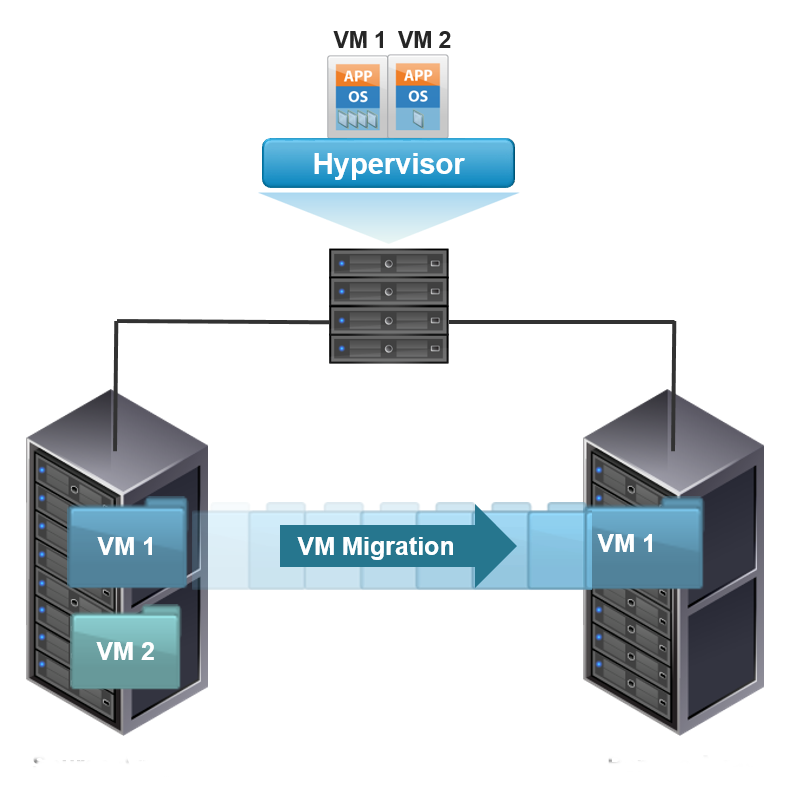
\includegraphics[width=250px]{img/vms_migration.eps}
 \caption{Live migration}
 Fonte: \citet{spaniol2015}
 \label{fig:vms_migration}
\end{figure}

Desta forma, obtem-se a alta disponibilidade dos serviços críticos da empresa a partir de um ambiente composto por \textit{softwares} de código 
aberto. Além disso, pode-se observar que existem uma variedade de ferramentas para atingir tal ojbetivo.

%pacemaker
% O \textit{Pacemaker}, irá eleger um nó como \textit{master}, para centralizar a gerência. Esse \textit{software} 
% também fará o monitoramento dos nós do \textit{cluster} e iniciará ou finalizará os serviços (recursos) em caso de falhas de um nó.
% ...
% 
% No \textit{Pacemaker}, os serviços que são configurados para serem monitorados são chamados de recursos (\textit{resources}).
% 
% Para configurar o ambiente deve-se criar esses recursos no \textit{Pacemaker}. Primeiramente deve-se criar o recurso para o \ac{DRBD}. 
% Esse recurso fará o monitoramento e fará a troca dos estados, primário e secundário, dos nós do \ac{DRBD}.
% Também será necessário criar um recurso para montar um sistema de arquivos para o dispositivo \ac{DRBD} no local onde ficarão os discos das 
% máquinas virtuais. Esse recurso executará juntamente com o recurso do \ac{DRBD}, assim, quando um nó do \ac{DRBD} for escolhido como primário 
% o sistema de arquivos será montado automaticamente.
% 
% E por fim, deve-se configurar um recurso para cada máquina virtual no \textit{Pacemaker} para possibilitar que as
% máquinas virtuais sejam migradas de um nó para outro de forma automática e transparente. 
% 
% Na configuração das máquinas virtuais, será ...
% De forma a balancear a carga do \textit{cluster}, as máquinas virtuais serão distribuídas entre os nós, ...


\section{Considerações finais}

Neste capítulo, foram apresentados os serviços críticos para a empresa. Além disso, foi apresentado uma proposta de solução. Destaca-se que 
durante o estudo das ferramentas foram realizados testes para uma melhor avaliação das mesmas.

